\documentclass{standalone}
\usepackage[utf8x]{inputenc}
\usepackage[T1]{fontenc}
\usepackage{libertine}
\usepackage{tikz}
\usetikzlibrary{trees,calc}
\begin{document}
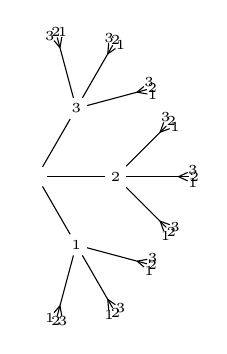
\begin{tikzpicture}[grow cyclic,
level 1/.style = {level distance = 1cm, sibling angle = 60},
level 2/.style = {level distance = .8cm, sibling angle = 45},
level 3/.style = {level distance = .2cm, sibling angle = 25}
]

%via three points = {one child at (0,1) and two children at (-1,1) and (1,1)}
%Distnacia entre la raíz y el nodo destino es 1cm
	%\node (R) at (0,0) {raíz} child; % Ramificación. 2 hijos, conviene usar \foreach
	%\node (r1) at (0,0) {R1} child child; % Las coordenadas apuntan al centro del nodo.
	%($(R) + (0,1.5)$)
\node at (0,0){}
	%\coordinate [rotate = 90; %]at (0,0);
	child foreach \i in {1, 2, 3}{
		node[fill = white, inner sep = 2pt]{\tiny{\i}}
		child  foreach \j in {1, 2, 3}{ % child {node {\i}}
			child foreach \k in {1, 2, 3}{
		node[inner sep = 0pt] {\tiny{\k}}
		}
	}
};
%\node 
\end{tikzpicture}
\end{document}
En el mapa mental se puede enlazar a un archivo.
Mediante el paquete ipref. Documentos dinámicos y referencias cruzadas.
Se gira en sentido horario, pero se puede definir en sentido antihorario.

Explicar cómo funciona foreach y los sistemas de coordenadas, ubicar un nodo respecto a otro.